\documentclass[conference]{IEEEtran}
\usepackage[USenglish]{babel}
\usepackage{graphicx}
\usepackage{cite}
\usepackage{amsmath}
\usepackage{graphicx}
\usepackage{graphics}
\usepackage{psfrag}
\usepackage{pstricks}
\usepackage{color}
\usepackage{amsmath}
\usepackage{rotating}
\usepackage{setspace}
\usepackage{cite} % ordena as citacoes
\usepackage[T1]{fontenc}
\usepackage{mathtools, cuted}
\ifCLASSINFOpdf
\else
% * <jose.avalos@utec.edu.pe> 2017-07-01T20:45:07.865Z:
%
% ^.
\fi
\hyphenation{op-tical net-works semi-conduc-tor}  

\begin{document}
%%%%%%%%%%%%%%%%%%%%% TITLE %%%%%%%%%%%%%%%%%%%%%%%%%%%%%%%%%%
\title{	Imitation of Human Drawing by a NAO Robot}
\author{\IEEEauthorblockN{Jose Maria Munoz\IEEEauthorrefmark{1}, Jose Avalos\IEEEauthorrefmark{1}
Oscar E. Ramos\IEEEauthorrefmark{1}}
\IEEEauthorblockA{\IEEEauthorrefmark{1}Department of Electrical Engineering, Universidad de Ingenieria y Tecnologia - UTEC, Lima, Peru.}
}
\maketitle
\begin{abstract}
Co-working applications are increasing in robotics due to the need of manipulating high volume of information in real time. This paper presents a methodology to develop a robot-based drawing system that allows the reproduction of an image shown by an operator. It incorporates cameras for real-time image processing, which uses filters, morphological operations and Hough transforms to obtain the desired features. A system calibration technique is also proposed to calibrate the coordinates of the robot with respect to the image frame before using an inverse kinematics method that controls the robot motion. The speed of the drawing imitation method depends on the network to which the system is connected. The proposed method is applied to the NAO robot and the framework consists of one robot being shown the desired image information while another robot, remotely localized, sketches the image.
\end{abstract}
\IEEEpeerreviewmaketitle
\textbf{\textit{Keywords - NAO robot, inverse kinematic, drawing robot.}}

\section{Introduction}
The robot NAO is a humanoid robot of 58 cm. height designed by the French company Aldebaran \cite{ref1}. The NAO has sensory functions similar to that of the
being human. If we classify the senses of the NAO, we can divide it into four parts: (a) Vision sensor, which helps the NAO to perceive the outside world, to be able to visualize, detect objects, recognize humans, etc. (b) Inertial Measurement Unit: This tells the NAO body its actual position. (c) Touch Sensor: This sends a signal to the NAO telling you that a part of your body has been touched and finally (d) Microphone: This allows you NOT to be able to communicate with people A complete description of the sensors, joints and links are can be seen in \cite{ref2}. In total, It has 25 degrees of freedom (DOF) (Head 2DOF, Arms (each) 5DOF, Pelvis 1DOF, Legs (each) 5DOF, Hands (each) 1DOF).

This paper demonstrates the ability of the NAO robot to be able to draw in coordination with the information obtained from its camera. According to the state art, the first humanoid that could be used as a draftsman was developed in EPFL with the help of the HOAP-2 robot \cite{ref3}. Robots can draw the drawing of anyone sitting in front of it. Primitive techniques for face detection, front edge detection and edge extraction along with trajectory planning. The other effort has been made by Srikaew \cite{ref4} to create artistic portraits using the ISAC robot. The good thing about using ISAC as a draftsman is because of his soft hands, since they can mitigate the drawing as fine as humans. They have an artificial McKibben muscle that is an actuator, while its stereo vision helps in the 3D rendering of the object. Paul a robotic system designed by \cite{ref5} draws the aesthetic human face more accurate than the aforementioned robots. This robot has four degrees of freedom with the camera placed on the body. It has an efficient control of feedback and extraction modules
of facial features.
\begin{center}	 
\includegraphics[scale=0.2]{nao.jpg}\\ 
\textbf{Figure.1} NAO Humanoid Robot
\end{center}

\section{Image Processing}
\label{sec:methodology}

This section explains the methods used for the processing of the images and thus obtain the necessary points to perform the inverse kinematics.

\subsection{Morphological Erosion}

To improve the quality of an image taken from the camera of the NAO, it is necessary to perform a pre-processing to the image. That is why a morphological operation will be used to increase the number of pixels and give a better quality to the image.It is the morphological transformation which combines two sets using the vector subtraction of set elements. If A and B are sets in Euclidean N-space, then the erosion of A by B is the set of all elements $x$ for which $x + b \in A$ for every $b \in B$. The erosion of A by B is denoted by $A \ominus B$ and is defined by:

\begin{equation}
\begin{split}
A \ominus B = &\{
x \in E^{N} \mid x + b \in  \textrm{A for every b}  \in B, \textrm{there exists an}\\
& \textrm{a} \in \textrm{A such that} x = a - b\}
\end{split}
\end{equation}
The utility of the erosion transformation is better appreciated when the erosion is expressed in a different form. The erosion of an image $A$ by a structuring element $B$ is the set of all elements $x$ of $E^{N}$ for which $B$ translated to $x$ is contained in $A$. In fact, this was the definition used for erosion by \cite{ref6}. The proof is immediate from the definition of erosion and the definition of translation.
\begin{equation}
A \ominus B =\{x \in E^{N} \mid (B)_{x} \subseteq A \}
\end{equation}
Thus the structuring element $B$ may be visualized as a probe which slides across the image $A$, testing the spatial nature of $A$ at every point. Where $B$ translated to $x$ can be contained in $A$ (by placing the origin of $B$ at $x$), then $x$ belongs to the erosion $A \ominus B$. 
Other proposition about erosion of an image A by structuring element B is the intersection af all translations of A by the points $-b$, where $b \in B$.
\begin{equation}
A \ominus B = \bigcap_{b \in B} (A)_{-b}
\end{equation}
\subsection{Canny edge detector}
Canny is an algorithm that is used to detect a wide range of edges in images. This algorithm is computationally eficient and is quite used for its good edge detection, good location and its minimum response.
The first stage to use Canny, is to use a filter based on the first derivative of a Gaussian to be able to reduce as much noise as possible. The result is a slightly blurred image compared to the original version.
The second step is to find the intensity of the gradient of the image; the edge of an image can point in different directions, so Canny's algorithm uses four filters to detect horizontal,vertical and diagonals edges of the blurred image. The edge detection operator (Roberts, Prewitt, Sobel) returns a value for the first derivative in the horizontal direction $(G_{y})$ and the vertical direction $(G_{x})$. From this, the edge gradient and the direction can be determined:
\begin{equation}
G = \sqrt{G_{x}^{2} + G_{y}^2}
\end{equation}
\begin{equation}
\Theta = \arctan(G_{y}/G_{x})
\end{equation}
\subsection{Hough Line Transform}
The Hough transform is used to detect edges more precisely. For this paper will be used to detect the lines. In the space of the image, the line can be represented by the equation:
\begin{equation}
y = m \times x + n
\end{equation}
and can be plotted for each pair $(x,y)$ of the image. In this algorithm, the main idea is consider the characteristics of a line in terms of its parameters $(m,n)$, and not as points of the image $(x_{1},y_{1}),\ldots,(x_{n},y_{n})$.Based on the above, the straight line $y = m \times x + n$ can be represented as a point $(m,n)$ in the parameter space. However, when vertical lines are present, the parameters of the line $(m,n)$ are indefinite. For this reason its better to use the parameters that describe a line in polar coordinates, denoted $(\rho, \theta)$. The parameter $\rho$ represents the distance between the origin of coordinates and the point $(x,y)$, while $\theta$ is the angle of the vector of the line perpendicular to the original line and passing through the coordinate origin. Using this parameterization, the equation of a line can be written as follows:
\begin{equation}
\label{1}
y = (\frac{-\cos\theta}{\sin\theta})\times x + (\frac{\rho}{\sin\theta})
\end{equation}
where the equation (\ref{1}) could be rewrite as:
\begin{equation}
\label{2}
\rho = x \times \cos\theta + y \times \sin\theta
\end{equation}

Then, it is possible to associate to each line a pair $(\rho,\theta)$ that is unique if $\theta \in [0,\pi)$ and $\rho \in \textbf{R}$ or $ \theta \in [0,2*\pi)$ and $\rho \geq 0$.The space $(\rho,\theta)$ is called the Hough space for the set lines in two dimensions. For an arbitrary point in the image with coordinates $(x_{0},y_{0})$, the lines passing through that point are the pairs $(\rho,\theta)$, in equation (\ref{2}) where $\rho$ (the distance between the straight line and the origin) is determined by $\theta$. This corresponds to a sinusoidal curve in space $(\rho,\theta)$, which is unique for that point. If the curves corresponding to two points intersect, the point of intersection in the Hough space corresponds to a line in the space of the image that passes through these two points. Generalizing, a set of points that form a line, will produce sinusoids that intersect in the parameters of that line.

\section{NAO Inverse Kinematics}
\subsection{Right Hand Inverse Kinematics}
Being a humanoid, the 'extremities' of the robot can be recognized, each, as independent kinematic chains. Each of these systems allows the accomplishment of different basic tasks such as standing, walking, sitting, among others. To have control over such tasks, it is necessary to know the inverse kinematics of each kinematic chain. Due to the activity in which we focus on this work, it is necessary to perform only the inverse kinematics of the kinematic chain corresponding to the right hand of the robot. Thus, we begin by defining the transformation matrix $T$:

\begin{equation}
T= 
\begin{pmatrix}
	r_{11}	& r_{12}	& r_{13}	&r_{14}\\
	r_{21}	& r_{22}	& r_{23}	&r_{24}\\
	r_{31}	& r_{32}	& r_{33}	&r_{34}\\
	0		& 0			& 0			& 1
\end{pmatrix}
\end{equation}

\begin{strip}
\begin{equation}
r_{11} = sin(\theta_{4})(sin(\theta_{1})sin(\hat{\theta_{3}})-cos(\theta_{1})cos(\hat{\theta_{2}})cos(\hat{\theta_{3}}))-cos(\theta_{1})cos(\theta_{4})sin(\hat{\theta_{2}})
\end{equation}

\begin{equation}
r_{12} = cos(\theta_{4})(sin(\theta_{1})sin(\hat{\theta_{3}})- cos(\theta_{1})cos(\hat{\theta_{2}})cos(\hat{\theta_{3}}))+ cos(\theta_{1})sin(\theta_{4})sin(\hat{\theta_{2}})\\
\end{equation}
\begin{equation}
r_{13} = cos(\hat{\theta_{3}})sin(\theta_{1})+cos(\theta_{1})-cos(\hat{\theta_{2}}sin(\hat{\theta_{3}}))\\
\end{equation}
\begin{equation}
r_{14} = l_{4}( sin(\theta_{4})( sin(\theta_{1})sin(\hat{\theta_{3}})- cos(\theta_{1})cos(\hat{\theta_{2}})cos(\hat{\theta_{3}}) ) )\\
\end{equation}
\begin{equation}
r_{21} = cos(\hat{\theta_{2}})cos(\theta_{4})- cos(\hat{\theta_{3}})sin(\hat{\theta_{2}})sin(\theta_{4})\\
\end{equation}
\begin{equation}
r_{22} = cos(\hat{\theta_{2}})sin(\theta_{4})- cos(\hat{\theta_{3}})sin(\hat{\theta_{2}})cos(\theta_{4})\\
\end{equation}
\begin{equation}
r_{23} = sin(\hat{\theta_{2}})sin(\hat{\theta_{3}})\\
\end{equation}
\begin{equation}
r_{24} = l_{1}+ l_{3}cos(\hat{\theta_{2}})+ l_{4}(cos(\hat{\theta_{2}})cos(\theta_{4})- cos(\hat{\theta_{3}})sin(\hat{\theta_{2}})sin(\theta_{4}))\\
\end{equation}
\begin{equation}
r_{31} = sin(\theta_{4})(  cos(\theta_{1})sin(\hat{\theta_{3}})+ cos(\hat{\theta_{2}})cos(\hat{\theta_{3}})sin(\theta_{1}))+ cos(\theta_{4})sin(\theta_{1})sin(\hat{\theta_{2}})\\
\end{equation}

\begin{equation}
r_{32} = cos(\theta_{4})(  cos(\theta_{1})sin(\hat{\theta_{3}})+ cos(\hat{\theta_{2}})cos(\hat{\theta_{3}})sin(\theta_{1}))- sin(\theta_{4})sin(\theta_{1})sin(\hat{\theta_{2}})\\
\end{equation}
\begin{equation}
r_{33} = cos(\theta_{1})cos(\hat{\theta_{3}})- cos(\hat{\theta_{2}})sin(\theta_1)sin(\hat{\theta_{3}})\\
\end{equation}

\begin{equation}
r_{34} = l_{2}+ l_{4}( sin(\theta_{4})(  cos(\theta_{1})sin(\hat{\theta_{3}})+cos(\hat{\theta_{2}})cos(\hat{\theta_{3}})sin(\theta_{1})  )+ cos(\theta_{4})sin(\theta_{1})sin(\hat{\theta_{2}})   )+ l_{3}sin(\theta_{1})sin(\hat{\theta_{2}})\\
\end{equation}
\end{strip}

\begin{strip}
where $\hat{\theta_{2}}$ represents the second joint. From this, due to the symmetry of both arms, we can define inverse kinetics as:
\end{strip}
\begin{strip}
\begin{equation}
\theta_{1}= \pm acos(\frac{T'_{(3,3)}+ \frac{T'_{(1,3)}sin(-\theta_{3})cos(\theta_{2}-\frac{pi}{2})}{cos(-\theta_{3})}}{cos(-\theta_{3})+ \frac{(cos(\theta_{2}-\frac{pi}{2}))^2(sin(-\theta_{3}))^2}{cos(-\theta_{3})}})\\
\end{equation}
\end{strip}
\begin{strip}
\begin{equation}
\theta_{1}= \pm acos(\frac{T'_{(1,3)}}{cos(\theta_{2}-\frac{\pi}{2})sin(-\theta_{3})})\\
\end{equation}
\end{strip}
\begin{strip}
\begin{equation}
\theta_{2}= \pm acos(\frac{T'_{(2,4)}-l_{1}-(\frac{l_{4}sin(\theta_{4})T'_{(2,2)}}{\cos(\theta_{4})})}{l_{3}+l_{4}cos(\theta_{4})+l_{4}\frac{(sin(\theta_{4}))^2}{cos(\theta_{4})}})\\
\end{equation}
\end{strip}
\begin{strip}
\begin{equation}
\theta_{3}= -asin(\frac{T'_{(2,3)}}{sin(\theta_{2}-\frac{\pi}{2})})\\
\end{equation}
\end{strip}
\begin{strip}
\begin{equation}
\theta_{3}= (\pi-asin(\frac{T'_{(2,3)}}{sin(\theta_{2}-\frac{\pi}{2})}))\\
\end{equation}
\end{strip}
\begin{strip}
\begin{equation}
\theta_{4}= (\pi-acos(\frac{l_{3}^2+l_{4}^2-\sqrt{(s_{x}-T'_{(1,4)})^2+(s_{y}-T'_{(2,4)})^2+(s_{z}-T'_{(3,4)})^2}^2}{2l_{3}l_{4}}))
\end{equation}
\end{strip}

\section{Methodology}
%\label{sec:methodology}

\begin{strip}
\begin{center}
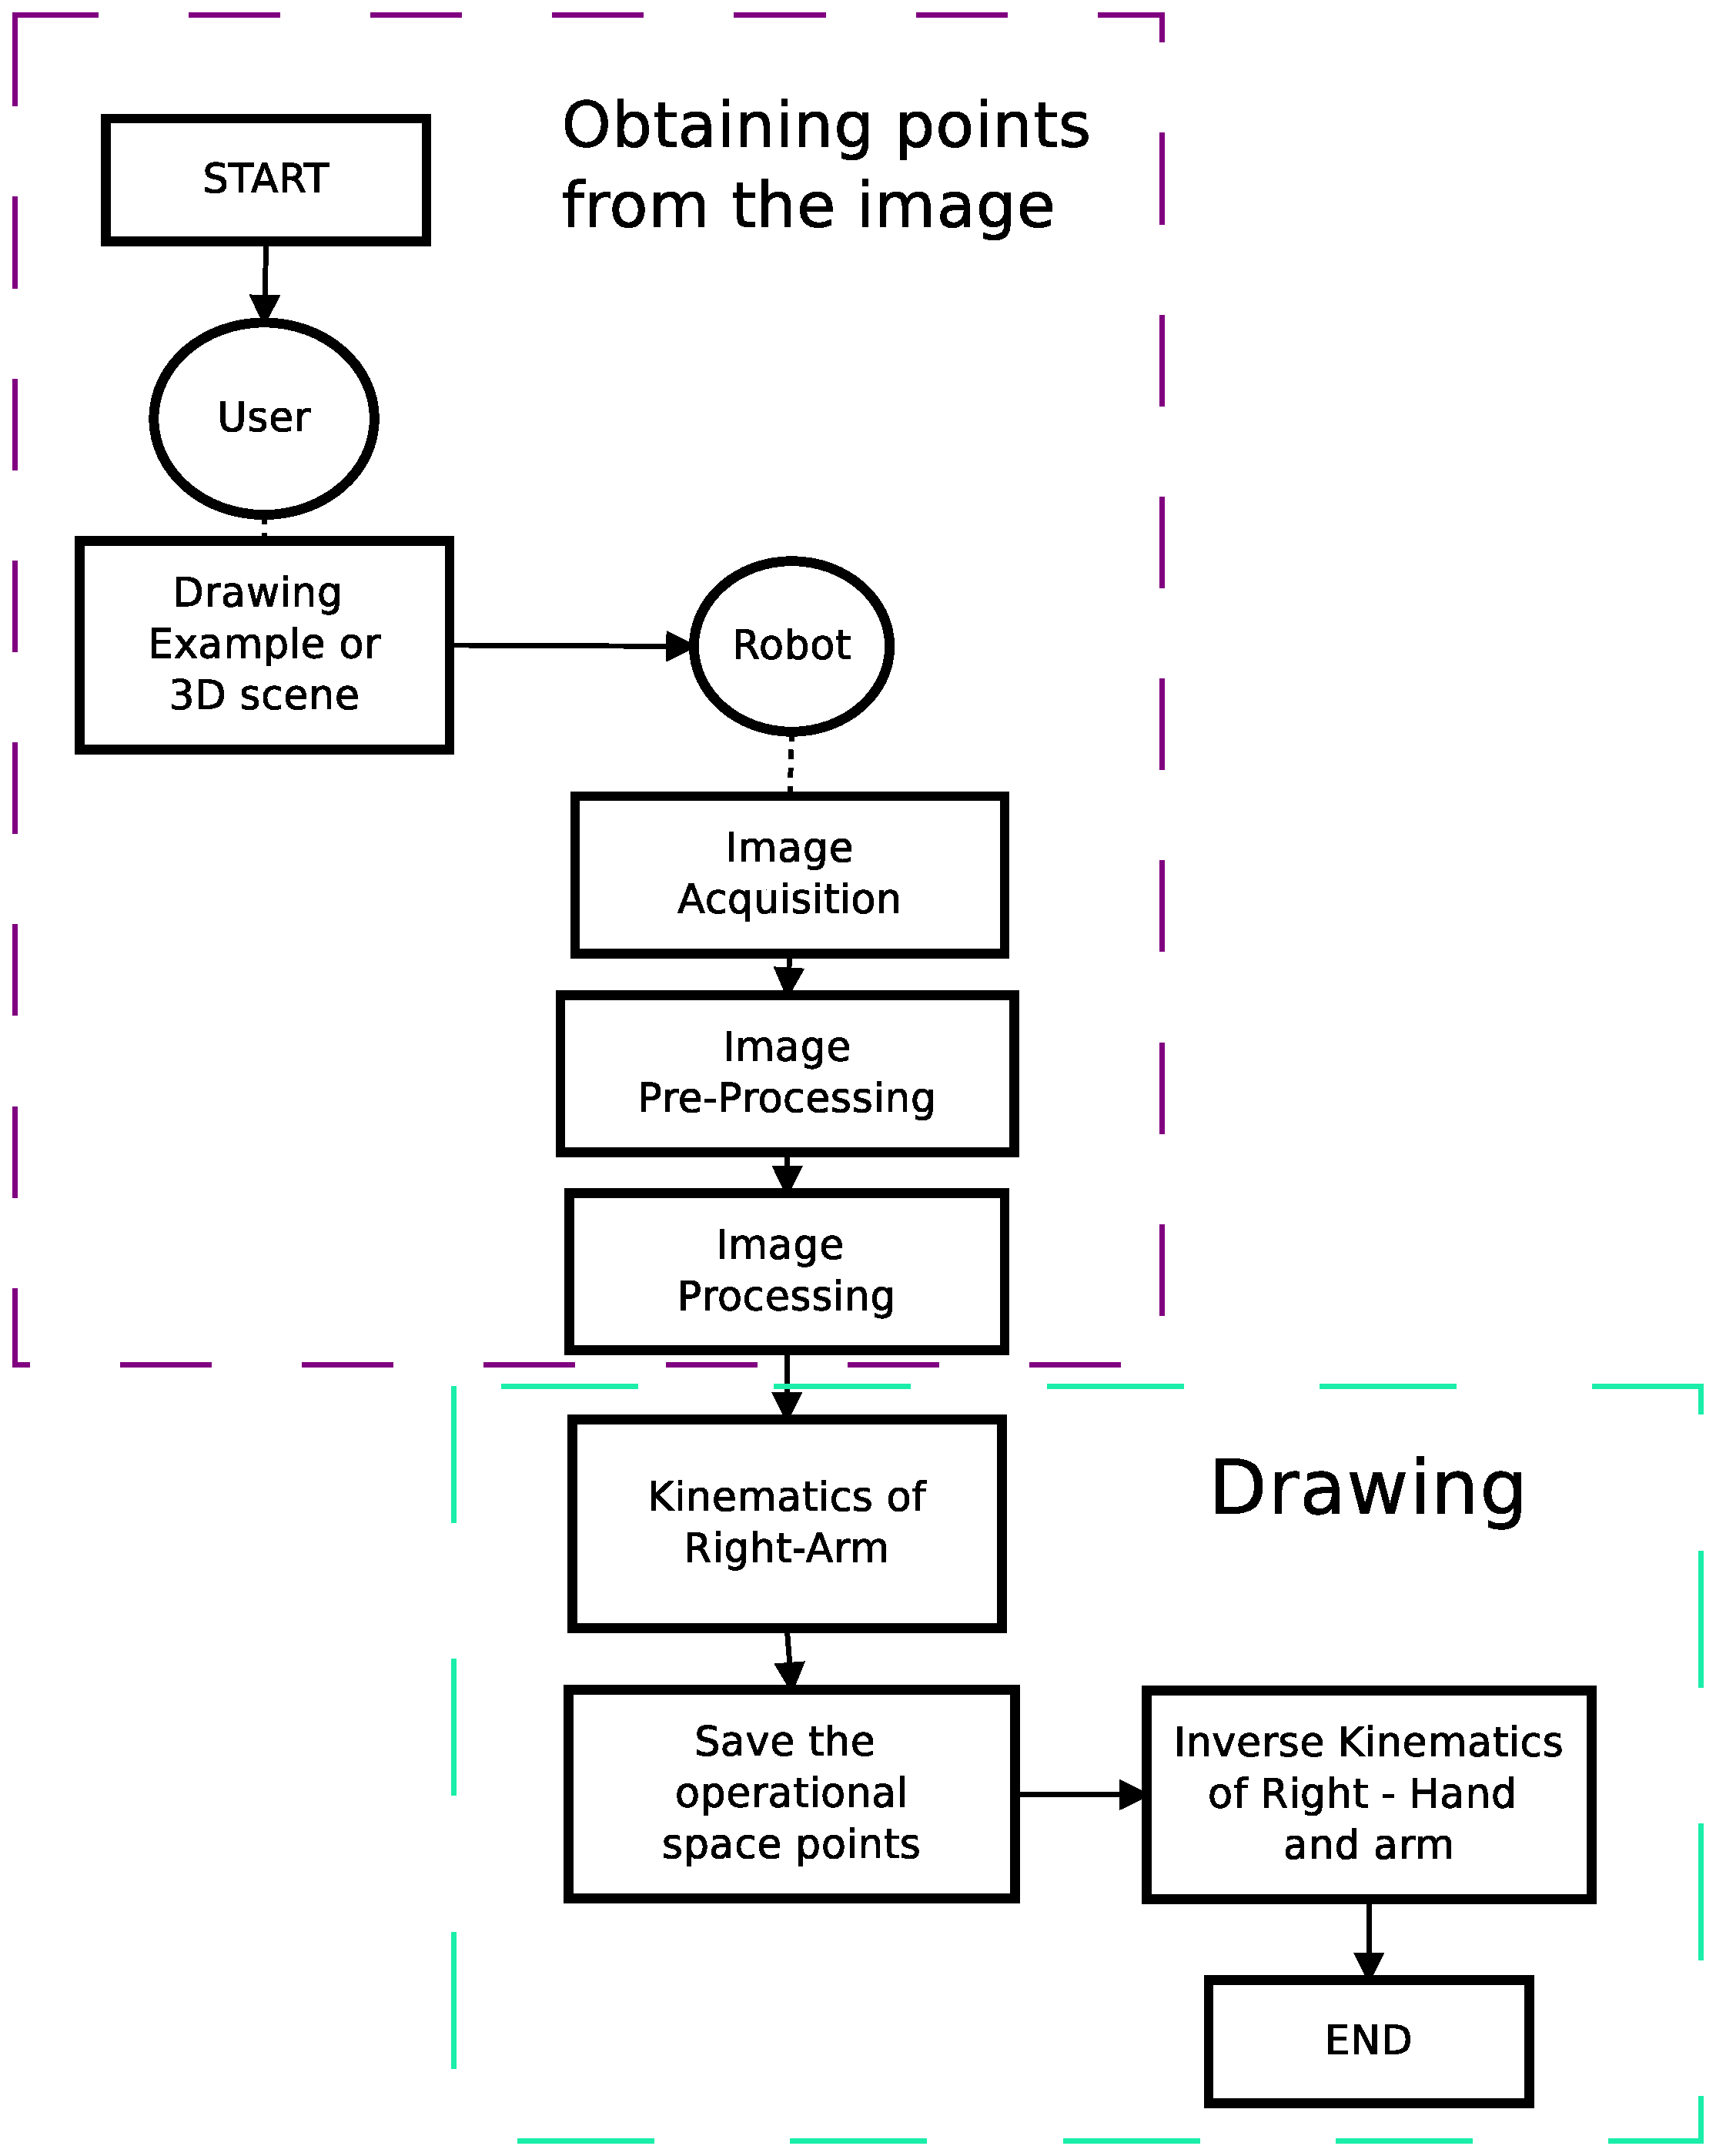
\includegraphics[scale=0.3]{flowchart.eps}\\
\textbf{Figure.2} Diagrama de Flujo para que el NAO pueda dibujar.
\end{center}
\end{strip}





\section{Conclusion}
\label{sec:conclusion}

% references section
\bibliographystyle{IEEEtran}
\bibliography{biblio.bib}
\end{document}
